%%%%%%%%%%%%%%%%%%%%%%%%%%%%%%%%%%%%%%%%%%%%%%%%%%%
\begin{frame}
  \begin{center}
    {\Large CNN with Keras: MNIST}
    
    {Ref: The Ultimate Beginner's Guide to Deep Learning in Python - EliteDataScience}
  \end{center}
\end{frame}

%%%%%%%%%%%%%%%%%%%%%%%%%%%%%%%%%%%%%%%%%%%%%%%%%%%
\begin{frame}[fragile] \frametitle{MNIST: Handwritten Digits Classification}
\begin{itemize}
\item Deep learning has led to major advances in computer vision. 
\item We're now able to classify images, find objects in them, and even label them with captions. 
\item To do so, deep neural networks with many hidden layers can sequentially learn more complex features from the raw input image
\end{itemize}
\end{frame}

%%%%%%%%%%%%%%%%%%%%%%%%%%%%%%%%%%%%%%%%%%%%%%%%%%%
\begin{frame}[fragile] \frametitle{Import Libraries}

\begin{itemize}
\item Importing numpy and setting a seed for the computer's pseudorandom number generator.
\begin{lstlisting}
import numpy as np
np.random.seed(123)  # for reproducibility
\end{lstlisting}
\item Keras libs
\begin{lstlisting}
from keras.models import Sequential
from keras.layers import Dense, Dropout, Activation, Flatten
from keras.layers import Conv2D, MaxPooling2D
\end{lstlisting}
\end{itemize}
\end{frame}

%%%%%%%%%%%%%%%%%%%%%%%%%%%%%%%%%%%%%%%%%%%%%%%%%%%
\begin{frame}[fragile] \frametitle{Load Data}

\begin{itemize}
\item MNIST is included in Keras
\item It's a big enough challenge to warrant neural networks, but it's manageable on a single computer. 
\end{itemize}
\begin{lstlisting}
from keras.datasets import mnist
 
# Load pre-shuffled MNIST data into train and test sets
(X_train, y_train), (X_test, y_test) = mnist.load_data()

print(X_train.shape)
# (60000, 28, 28)
print(X_train[0].shape)
# (26,28)
\end{lstlisting}
We have 60,000 samples in our training set, and the images are 28 pixels x 28 pixels each.
\end{frame}

%%%%%%%%%%%%%%%%%%%%%%%%%%%%%%%%%%%%%%%%%%%%%%%%%%%
\begin{frame}[fragile] \frametitle{Load Data}

\begin{itemize}
\item Check by plotting a sample image
\end{itemize}
\begin{lstlisting}
from matplotlib import pyplot as plt
plt.imshow(X_train[0])
plt.show()
\end{lstlisting}
\begin{center}
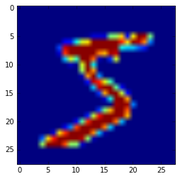
\includegraphics[width=0.3\linewidth,keepaspectratio]{cnnkr2}
\end{center}
\end{frame}

%%%%%%%%%%%%%%%%%%%%%%%%%%%%%%%%%%%%%%%%%%%%%%%%%%%
\begin{frame}[fragile] \frametitle{Input Shape}

\begin{itemize}
\item If your image batch is of N images of HxW size with C channels, theano uses the NCHW ordering while tensorflow uses the NHWC ordering.
\item This example shows TH way of ordering
\item For TF way, you can either change it to 
\begin{lstlisting}
X_train = X_train.reshape(X_train.shape[0], img_cols, img_rows, 1)
X_test = X_test.reshape(X_test.shape[0], img_cols, img_rows, 1)
input_shape=(img_cols, img_rows, 1)
\end{lstlisting}
\item or say
\begin{lstlisting}
from keras import backend as K
K.set_image_dim_ordering('th')
\end{lstlisting}
\end{itemize}
\end{frame}



%%%%%%%%%%%%%%%%%%%%%%%%%%%%%%%%%%%%%%%%%%%%%%%%%%%
\begin{frame}[fragile] \frametitle{Input Shape in MNIST}

\begin{itemize}
\item A full-color image with all 3 RGB channels will have a depth of 3.
\item Our MNIST images only have a depth of 1
\item We want to transform our dataset from having shape (n, width, height) to (n, width, height, depth) in \lstinline|data_format= "channels_last"|.
\end{itemize}
\begin{lstlisting}
keras.backend.set_image_data_format('channels_last')
X_train = X_train.reshape(X_train.shape[0], 28, 28, 1)
X_test = X_test.reshape(X_test.shape[0], 28, 28, 1)
print(X_train.shape)
# (60000, 1, 28, 28)
\end{lstlisting}
\end{frame}


%%%%%%%%%%%%%%%%%%%%%%%%%%%%%%%%%%%%%%%%%%%%%%%%%%%
\begin{frame}[fragile] \frametitle{Pre-process Data}

\begin{itemize}
\item Convert our data type to float32
\item Normalize our data values to the range [0, 1].
\end{itemize}
\begin{lstlisting}
X_train = X_train.astype('float32')
X_test = X_test.astype('float32')
X_train /= 255
X_test /= 255
\end{lstlisting}
Now, our input data Xs are ready for model training.
\end{frame}

%%%%%%%%%%%%%%%%%%%%%%%%%%%%%%%%%%%%%%%%%%%%%%%%%%%
\begin{frame}[fragile] \frametitle{Pre-process Labels}

\begin{itemize}
\item Let's take a look at the shape of our class label data:
\begin{lstlisting}
print(y_train.shape)
# (60000,)
\end{lstlisting}
\item That may be problematic. 
\item We should have 10 different classes, one for each digit, but it looks like we only have a 1-dimensional array.
\item Let's take a look at the labels for the first 10 training samples:
\begin{lstlisting}
print(y_train[:10])
# [5 0 4 1 9 2 1 3 1 4]
\end{lstlisting}
\end{itemize}
\end{frame}


%%%%%%%%%%%%%%%%%%%%%%%%%%%%%%%%%%%%%%%%%%%%%%%%%%%
\begin{frame}[fragile] \frametitle{Pre-process Labels}

\begin{itemize}
\item And there's the problem. 
\item The y\_train and y\_test data are not split into 10 distinct class labels, but rather are represented as a single array with the class values.
\item We can fix this easily:
\begin{lstlisting}
from keras.utils import to_categorical

# Convert 1-dimensional class arrays to 10-dimensional class matrices
Y_train = to_categorical(y_train)
Y_test = to_categorical(y_test)
\end{lstlisting}
\item See now:
\begin{lstlisting}
print(Y_train.shape)
# (60000, 10)
\end{lstlisting}
\end{itemize}
\end{frame}


%%%%%%%%%%%%%%%%%%%%%%%%%%%%%%%%%%%%%%%%%%%%%%%%%%%
\begin{frame}[fragile] \frametitle{Define Model}

\begin{itemize}
\item The input shape parameter should be the shape of 1 sample. 
\item In this case, it's the same (28, 28, 1) that corresponds to  the (width, height,depth) of each digit image.
\item But what do the first 3 parameters represent? 
\item They correspond to the number of convolution filters to use, the number of rows in each convolution kernel, and the number of columns in each convolution kernel, respectively.
\item We can confirm this by printing the shape of the current model output:
\end{itemize}
\begin{lstlisting}
model = Sequential()
model.add(Conv2D(32,  kernel_size=3, activation='relu', input_shape=(28,28,1)))
print(model.output_shape)
# (None, 32, 26, 26)
\end{lstlisting}
*Note: The step size is (1,1) by default, and it can be tuned using the 'subsample' parameter.
\end{frame}



%%%%%%%%%%%%%%%%%%%%%%%%%%%%%%%%%%%%%%%%%%%%%%%%%%%
\begin{frame}[fragile] \frametitle{Conv2D output size}

\begin{itemize}
\item Tensor size or shape: (width = 28, height = 28)
\item Convolution filter size (F): (F\_width = 3, F\_height = 3)
\item Padding (P): 0
\item Stride (S): 1
\item Using the equation:
\item output width=$((W-F+2*P )/S)+ 1 = ((28-3+2*0)/1) + 1 = 26$
\end{itemize}


\end{frame}


%%%%%%%%%%%%%%%%%%%%%%%%%%%%%%%%%%%%%%%%%%%%%%%%%%%
\begin{frame}[fragile] \frametitle{Pooling}

\begin{itemize}
\item We can simply add more layers to our model like we're building legos.
\item Dropout is a method for regularizing our model in order to prevent overfitting. 
\item Let also remember that a pooling is a form of "filter" and thus the $((W-F+2*P )/S)+ 1$ equation is a applicable.
\item So after max pooling of $2x2$ with Stride 2, it will be $=(((W-F+2*P )/S)+1) = (((26-2+2*0)/2)+1 = 13$
\end{itemize}
\begin{lstlisting}
model.add(MaxPooling2D(pool_size=(2,2)))
model.add(Dropout(0.25))
\end{lstlisting}

\end{frame}

%%%%%%%%%%%%%%%%%%%%%%%%%%%%%%%%%%%%%%%%%%%%%%%%%%%
\begin{frame}[fragile] \frametitle{Define Model}

\begin{itemize}
\item For Dense layers, the first parameter is the output size of the layer. Keras automatically handles the connections between layers.
\item Note that the final layer has an output size of 10, corresponding to the 10 classes of digits.
\item Also note that the weights from the Convolution layers must be flattened (made 1-dimensional) before passing them to the fully connected Dense layer.
\end{itemize}
\begin{lstlisting}
model.add(Flatten())
model.add(Dense(128, activation='relu'))
model.add(Dropout(0.5))
model.add(Dense(10, activation='softmax'))
\end{lstlisting}
\end{frame}

%%%%%%%%%%%%%%%%%%%%%%%%%%%%%%%%%%%%%%%%%%%%%%%%%%%
\begin{frame}[fragile] \frametitle{Compile Model}

\begin{itemize}
\item We just need to compile the model and we'll be ready to train it. 
\item When we compile the model, we declare the loss function and the optimizer (SGD, Adam, etc.).
\item Keras has a variety of loss functions and out-of-the-box optimizers to choose from.
\end{itemize}
\begin{lstlisting}
model.compile(loss='categorical_crossentropy',
              optimizer='adam',
              metrics=['accuracy'])
\end{lstlisting}
\end{frame}

%%%%%%%%%%%%%%%%%%%%%%%%%%%%%%%%%%%%%%%%%%%%%%%%%%%
\begin{frame}[fragile] \frametitle{Fit Model}

\begin{itemize}
\item To fit the model, all we have to do is declare the batch size and number of epochs to train for, 
\item Then pass in our training data.
\end{itemize}
\begin{lstlisting}
model.fit(X_train, Y_train, 
          batch_size=32, nb_epoch=10, verbose=1)
\end{lstlisting}
You can also use a variety of callbacks to set early-stopping rules, save model weights along the way, or log the history of each training epoch.
\end{frame}

%%%%%%%%%%%%%%%%%%%%%%%%%%%%%%%%%%%%%%%%%%%%%%%%%%%
\begin{frame}[fragile] \frametitle{Evaluate Model}
We can evaluate our model on the test data.
\begin{lstlisting}
score = model.evaluate(X_test, Y_test, verbose=0)
print(score)
0.9855
\end{lstlisting}

\end{frame}



%%%%%%%%%%%%%%%%%%%%%%%%%%%%%%%%%%%%%%%%%%%%%%%%%%%
\begin{frame}
  \begin{center}
    {\Large CNN with Keras: CIFAR-10}
    
    {Ref: Machine Learning Mastery - Jason Brownlee}
  \end{center}
\end{frame}

%%%%%%%%%%%%%%%%%%%%%%%%%%%%%%%%%%%%%%%%%%%%%%%%%%%
\begin{frame}[fragile] \frametitle{The CIFAR-10 Problem Description}
\begin{itemize}
\item The problem of automatically identifying objects in photographs is difficult because of the near infinite number of permutations of objects, positions, lighting and so on. 
\item It's a really hard problem.
\item  A standard computer vision and deep learning dataset for this problem was developed by the Canadian Institute for Advanced Research (CIFAR).
\end{itemize}
\end{frame}


%%%%%%%%%%%%%%%%%%%%%%%%%%%%%%%%%%%%%%%%%%%%%%%%%%%
\begin{frame}[fragile] \frametitle{The CIFAR-10 Problem Description}

\begin{itemize}
\item The CIFAR-10 dataset consists of 60,000 photos divided into 10 classes (hence the name CIFAR-10). 
\item Classes include common objects such as airplanes, automobiles, birds, cats and so on. 
\item The dataset is split in a standard way, where 50,000 images are used for training a model and the remaining 10,000 for evaluating its performance.
\item The photos are in color with red, green and blue components, but are small measuring 32 by 32 pixel squares.
\end{itemize}
\end{frame}


%%%%%%%%%%%%%%%%%%%%%%%%%%%%%%%%%%%%%%%%%%%%%%%%%%%
\begin{frame}[fragile] \frametitle{Loading The CIFAR-10 Dataset in Keras}

\begin{lstlisting}
from keras.datasets import cifar10
from matplotlib import pyplot
from scipy.misc import toimage

# load data
(X_train, y_train), (X_test, y_test) = cifar10.load_data()

# create a grid of 3x3 images
for i in range(0, 9):
    pyplot.subplot(330 + 1 + i)
    pyplot.imshow(toimage(X_train[i]))
    
# show the plot
pyplot.show()
\end{lstlisting}
Running the code create a 3x3 plot of photographs.
\end{frame}


%%%%%%%%%%%%%%%%%%%%%%%%%%%%%%%%%%%%%%%%%%%%%%%%%%%
\begin{frame}[fragile] \frametitle{Loading The CIFAR-10 Dataset in Keras}
\begin{itemize}
\item The images have been scaled up from their small 32x32 size, but you can clearly see trucks horses and cars.
\item You can also see some distortion in some images that have been forced to the square aspect ratio.
\end{itemize}
\begin{center}
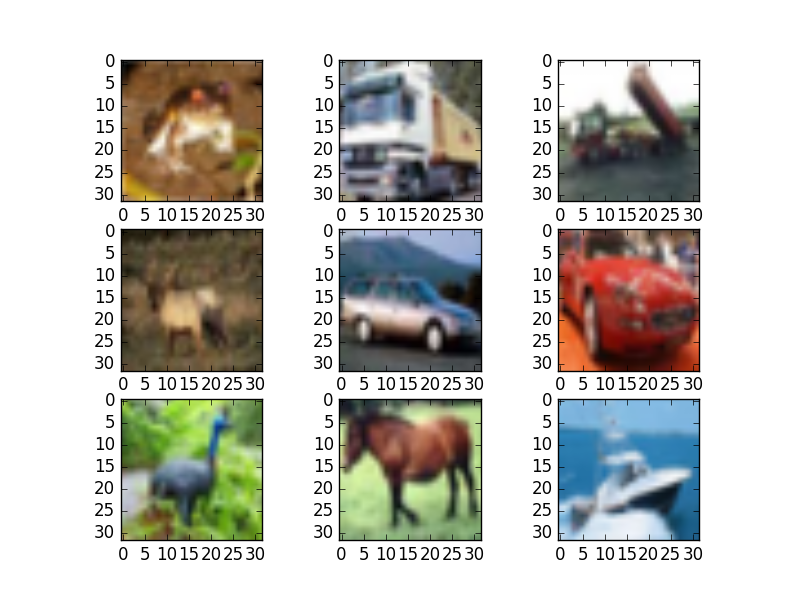
\includegraphics[width=0.7\linewidth,keepaspectratio]{cnnkr1}
\end{center}
\end{frame}



%%%%%%%%%%%%%%%%%%%%%%%%%%%%%%%%%%%%%%%%%%%%%%%%%%%
\begin{frame}[fragile] \frametitle{Simple Convolutional Neural Network for CIFAR-10}
Imports:
\begin{lstlisting}
# Simple CNN model for CIFAR-10
import numpy
from keras.datasets import cifar10
from keras.models import Sequential
from keras.layers import Dense
from keras.layers import Dropout
from keras.layers import Flatten
from keras.constraints import maxnorm
from keras.optimizers import SGD
from keras.layers.convolutional import Conv2D
from keras.layers.convolutional import MaxPooling2D
from keras.utils import np_utils
from keras import backend as K
K.set_image_dim_ordering('th')
\end{lstlisting}

\end{frame}

%%%%%%%%%%%%%%%%%%%%%%%%%%%%%%%%%%%%%%%%%%%%%%%%%%%
\begin{frame}[fragile] \frametitle{Simple Convolutional Neural Network for CIFAR-10}
As is good practice, we next initialize the random number seed with a constant to ensure the results are reproducible.
\begin{lstlisting}
# fix random seed for reproducibility
seed = 7
numpy.random.seed(seed)
\end{lstlisting}
Next we can load the CIFAR-10 dataset.
\begin{lstlisting}
# load data
(X_train, y_train), (X_test, y_test) = cifar10.load_data()
\end{lstlisting}
\end{frame}

%%%%%%%%%%%%%%%%%%%%%%%%%%%%%%%%%%%%%%%%%%%%%%%%%%%
\begin{frame}[fragile] \frametitle{Simple Convolutional Neural Network for CIFAR-10}
\begin{itemize}
\item The pixel values are in the range of 0 to 255 for each of the red, green and blue channels.
\item It is good practice to work with normalized data to the range 0 to 1 by dividing each value by the maximum observation which is 255.
\item Note, the data is loaded as integers, so we must cast it to floating point values in order to perform the division.
\end{itemize}
\begin{lstlisting}
# normalize inputs from 0-255 to 0.0-1.0
X_train = X_train.astype('float32')
X_test = X_test.astype('float32')
X_train = X_train / 255.0
X_test = X_test / 255.0
\end{lstlisting}
\end{frame}

%%%%%%%%%%%%%%%%%%%%%%%%%%%%%%%%%%%%%%%%%%%%%%%%%%%
\begin{frame}[fragile] \frametitle{Simple Convolutional Neural Network for CIFAR-10}
\begin{itemize}
\item The output variables are defined as a vector of integers from 0 to 1 for each class.
\item We can use a one hot encoding to transform them into a binary matrix in order to best model the classification problem. 
\item We know there are 10 classes for this problem, so we can expect the binary matrix to have a width of 10.
\end{itemize}
\begin{lstlisting}
# one hot encode outputs
y_train = np_utils.to_categorical(y_train)
y_test = np_utils.to_categorical(y_test)
num_classes = y_test.shape[1]
\end{lstlisting}
\end{frame}

%%%%%%%%%%%%%%%%%%%%%%%%%%%%%%%%%%%%%%%%%%%%%%%%%%%
\begin{frame}[fragile] \frametitle{Simple Convolutional Neural Network for CIFAR-10}
\begin{itemize}
\item Start off by defining a simple CNN structure as a baseline and evaluate how well it performs on the problem.
\item We will use a structure with two convolutional layers followed by max pooling and a flattening out of the network to fully connected layers to make predictions.
\end{itemize}
\end{frame}

%%%%%%%%%%%%%%%%%%%%%%%%%%%%%%%%%%%%%%%%%%%%%%%%%%%
\begin{frame}[fragile] \frametitle{Simple Convolutional Neural Network for CIFAR-10}
Our baseline network structure can be summarized as follows:
\begin{itemize}
\item Convolutional input layer, 32 feature maps with a size of 3x3, a rectifier activation function and a weight constraint of max norm set to 3.
\item     Dropout set to 20\%.
\item     Convolutional layer, 32 feature maps with a size of 3x3, a rectifier activation function and a weight constraint of max norm set to 3.
\item     Max Pool layer with size 2x2.
\item     Flatten layer.
\item     Fully connected layer with 512 units and a rectifier activation function.
\item     Dropout set to 50\%.
\item     Fully connected output layer with 10 units and a softmax activation function.

\end{itemize}
\end{frame}

%%%%%%%%%%%%%%%%%%%%%%%%%%%%%%%%%%%%%%%%%%%%%%%%%%%
\begin{frame}[fragile] \frametitle{Simple Convolutional Neural Network for CIFAR-10}
\begin{lstlisting}
# Create the model
model = Sequential()
model.add(Conv2D(32,  kernel_size=3, input_shape=(32, 32,3), padding='same', activation='relu', kernel_constraint=maxnorm(3)))
model.add(Dropout(0.2))
model.add(Conv2D(32, kernel_size=3, activation='relu', padding='same', kernel_constraint=maxnorm(3)))
model.add(MaxPooling2D(pool_size=(2, 2)))
model.add(Flatten())
model.add(Dense(512, activation='relu', kernel_constraint=maxnorm(3)))
model.add(Dropout(0.5))
model.add(Dense(num_classes, activation='softmax'))
\end{lstlisting}

*Note: \lstinline|kernel_constraint=maxnorm(3)| Constrains the weights incident to each hidden unit to have a norm less than or equal to a desired value ie 3, here, to avoid overfitting.
\end{frame}

%%%%%%%%%%%%%%%%%%%%%%%%%%%%%%%%%%%%%%%%%%%%%%%%%%%
\begin{frame}[fragile] \frametitle{Simple Convolutional Neural Network for CIFAR-10}
A logarithmic loss function is used with the stochastic gradient descent optimization algorithm configured with a large momentum and weight decay start with a learning rate of 0.01.
\begin{lstlisting}
# Compile model
epochs = 25
lrate = 0.01
decay = lrate/epochs
sgd = SGD(lr=lrate, momentum=0.9, decay=decay, nesterov=False)
model.compile(loss='categorical_crossentropy', optimizer=sgd, metrics=['accuracy'])
print(model.summary())
\end{lstlisting}
We can fit this model with 25 epochs and a batch size of 32.
\end{frame}

%%%%%%%%%%%%%%%%%%%%%%%%%%%%%%%%%%%%%%%%%%%%%%%%%%%
\begin{frame}[fragile] \frametitle{Simple Convolutional Neural Network for CIFAR-10}

\begin{itemize}
\item A small number of epochs was chosen to help keep this tutorial moving. 
\item Normally the number of epochs would be one or two orders of magnitude larger for this problem.
\item Once the model is fit, we evaluate it on the test dataset and print out the classification accuracy.
\end{itemize}
\begin{lstlisting}
# Fit the model
model.fit(X_train, y_train, validation_data=(X_test, y_test), epochs=epochs, batch_size=32)
# Final evaluation of the model
scores = model.evaluate(X_test, y_test, verbose=0)
print("Accuracy: %.2f%%" % (scores[1]*100))
\end{lstlisting}
\end{frame}

%%%%%%%%%%%%%%%%%%%%%%%%%%%%%%%%%%%%%%%%%%%%%%%%%%%
\begin{frame}[fragile] \frametitle{Simple Convolutional Neural Network for CIFAR-10}

\begin{itemize}
\item Running this example provides the results below. 
\item First the network structure is summarized which confirms our design was implemented correctly.
\end{itemize}
\begin{lstlisting}
_________________________________________________________________
Layer (type)                 Output Shape              Param #  
=================================================================
conv2d_1 (Conv2D)            (None, 32, 32, 32)        896      
_________________________________________________________________
dropout_1 (Dropout)          (None, 32, 32, 32)        0        
_________________________________________________________________
conv2d_2 (Conv2D)            (None, 32, 32, 32)        9248      
_________________________________________________________________
\end{lstlisting}
\end{frame}

%%%%%%%%%%%%%%%%%%%%%%%%%%%%%%%%%%%%%%%%%%%%%%%%%%%
\begin{frame}[fragile] \frametitle{Simple Convolutional Neural Network for CIFAR-10}

\begin{lstlisting}
_________________________________________________________________
max_pooling2d_1 (MaxPooling2 (None, 32, 16, 16)        0        
_________________________________________________________________
flatten_1 (Flatten)          (None, 8192)              0        
_________________________________________________________________
dense_1 (Dense)              (None, 512)               4194816  
_________________________________________________________________
dropout_2 (Dropout)          (None, 512)               0        
_________________________________________________________________
dense_2 (Dense)              (None, 10)                5130      
=================================================================
\end{lstlisting}
\end{frame}


%%%%%%%%%%%%%%%%%%%%%%%%%%%%%%%%%%%%%%%%%%%%%%%%%%%
\begin{frame}[fragile] \frametitle{Simple Convolutional Neural Network for CIFAR-10}
\begin{itemize}
\item The classification accuracy and loss is printed each epoch on both the training and test datasets. 
\item The model is evaluated on the test set and achieves an accuracy of 70.85\%, which is not excellent.
\end{itemize}
\begin{lstlisting}
Total params: 4,210,090.0
Trainable params: 4,210,090.0
Non-trainable params: 0.0
\end{lstlisting}
\end{frame}

%%%%%%%%%%%%%%%%%%%%%%%%%%%%%%%%%%%%%%%%%%%%%%%%%%%
\begin{frame}[fragile] \frametitle{Simple Convolutional Neural Network for CIFAR-10}
\begin{lstlisting}
Epoch 23/25
50000/50000 [==============================] - 143s - loss: 0.2399 - acc: 0.9168 - val_loss: 1.0680 - val_acc: 0.7077
Epoch 24/25
50000/50000 [==============================] - 143s - loss: 0.2285 - acc: 0.9197 - val_loss: 1.0702 - val_acc: 0.7119
Epoch 25/25
50000/50000 [==============================] - 143s - loss: 0.2177 - acc: 0.9238 - val_loss: 1.0686 - val_acc: 0.7085
Accuracy: 70.85%
\end{lstlisting}
We can improve the accuracy significantly by creating a much deeper network. 
\end{frame}

%%%%%%%%%%%%%%%%%%%%%%%%%%%%%%%%%%%%%%%%%%%%%%%%%%%
\begin{frame}[fragile] \frametitle{Larger Convolutional Neural Network for CIFAR-10}
\begin{itemize}
\item We can introduce an additional round of convolutions with many more feature maps. 
\item We will use the same pattern of Convolutional, Dropout, Convolutional and Max Pooling layers.
\item This pattern will be repeated 3 times with 32, 64, and 128 feature maps. 
\item The effect be an increasing number of feature maps with a smaller and smaller size given the max pooling layers. Finally an additional and larger Dense layer will be used at the output end of the network in an attempt to better translate the large number feature maps to class values.
\end{itemize}
\end{frame}

%%%%%%%%%%%%%%%%%%%%%%%%%%%%%%%%%%%%%%%%%%%%%%%%%%%
\begin{frame}[fragile] \frametitle{Larger Convolutional Neural Network for CIFAR-10}
We can summarize a new network architecture as follows:
\begin{itemize}
\item Convolutional input layer, 32 feature maps with a size of 3x3 and a rectifier activation function.
\item Dropout layer at 20\%.
\item Convolutional layer, 32 feature maps with a size of 3x3 and a rectifier activation function.
\item Max Pool layer with size 2x2.
\item Convolutional layer, 64 feature maps with a size of 3x3 and a rectifier activation function.
\item Dropout layer at 20\%.
\item Convolutional layer, 64 feature maps with a size of 3x3 and a rectifier activation function.
\item Max Pool layer with size 2x2.
\item Convolutional layer, 128 feature maps with a size of 3x3 and a rectifier activation function.
\item Dropout layer at 20\%.
\end{itemize}
\end{frame}

%%%%%%%%%%%%%%%%%%%%%%%%%%%%%%%%%%%%%%%%%%%%%%%%%%%
\begin{frame}[fragile] \frametitle{Larger Convolutional Neural Network for CIFAR-10}

\begin{itemize}
\item Convolutional layer,128 feature maps with a size of 3x3 and a rectifier activation function.
\item Max Pool layer with size 2x2.
\item Flatten layer.
\item Dropout layer at 20\%.
\item Fully connected layer with 1024 units and a rectifier activation function.
\item Dropout layer at 20\%.
\item Fully connected layer with 512 units and a rectifier activation function.
\item Dropout layer at 20\%.
\item Fully connected output layer with 10 units and a softmax activation function
\end{itemize}
\end{frame}


%%%%%%%%%%%%%%%%%%%%%%%%%%%%%%%%%%%%%%%%%%%%%%%%%%%
\begin{frame}[fragile] \frametitle{Simple Convolutional Neural Network for CIFAR-10}
We can very easily define this network topology in Keras, as follows:
\begin{lstlisting}
# Create the model
model = Sequential()
model.add(Conv2D(32,  kernel_size=3, input_shape=(32, 32,3), activation='relu', padding='same'))
model.add(Dropout(0.2))
model.add(Conv2D(32,  kernel_size=3, activation='relu', padding='same'))
model.add(MaxPooling2D(pool_size=(2, 2)))
model.add(Conv2D(64,  kernel_size=3, activation='relu', padding='same'))
model.add(Dropout(0.2))
model.add(Conv2D(64,  kernel_size=3, activation='relu', padding='same'))
model.add(MaxPooling2D(pool_size=(2, 2)))
model.add(Conv2D(128,  kernel_size=3, activation='relu', padding='same'))
model.add(Dropout(0.2))
\end{lstlisting}

\end{frame}

%%%%%%%%%%%%%%%%%%%%%%%%%%%%%%%%%%%%%%%%%%%%%%%%%%%
\begin{frame}[fragile] \frametitle{Simple Convolutional Neural Network for CIFAR-10}
\begin{lstlisting}
model.add(Conv2D(128, kernel_size=3, activation='relu', padding='same'))
model.add(MaxPooling2D(pool_size=(2, 2)))
model.add(Flatten())
model.add(Dropout(0.2))
model.add(Dense(1024, activation='relu', kernel_constraint=maxnorm(3)))
model.add(Dropout(0.2))
model.add(Dense(512, activation='relu', kernel_constraint=maxnorm(3)))
model.add(Dropout(0.2))
model.add(Dense(num_classes, activation='softmax'))
\end{lstlisting}

\end{frame}

%%%%%%%%%%%%%%%%%%%%%%%%%%%%%%%%%%%%%%%%%%%%%%%%%%%
\begin{frame}[fragile] \frametitle{Simple Convolutional Neural Network for CIFAR-10}
\begin{lstlisting}
# Compile model
epochs = 25
lrate = 0.01
decay = lrate/epochs
sgd = SGD(lr=lrate, momentum=0.9, decay=decay, nesterov=False)
model.compile(loss='categorical_crossentropy', optimizer=sgd, metrics=['accuracy'])
print(model.summary())
\end{lstlisting}

\end{frame}

%%%%%%%%%%%%%%%%%%%%%%%%%%%%%%%%%%%%%%%%%%%%%%%%%%%
\begin{frame}[fragile] \frametitle{Simple Convolutional Neural Network for CIFAR-10}
We can fit and evaluate this model using the same a procedure above and the same number of epochs but a larger batch size of 64, found through some minor experimentation.
\begin{lstlisting}
numpy.random.seed(seed)
model.fit(X_train, y_train, validation_data=(X_test, y_test), epochs=epochs, batch_size=64)
# Final evaluation of the model
scores = model.evaluate(X_test, y_test, verbose=0)
print("Accuracy: %.2f%%" % (scores[1]*100))
\end{lstlisting}

\end{frame}

%%%%%%%%%%%%%%%%%%%%%%%%%%%%%%%%%%%%%%%%%%%%%%%%%%%
\begin{frame}[fragile] \frametitle{Larger Convolutional Neural Network for CIFAR-10}
\begin{itemize}
\item Running this example prints the classification accuracy and loss on the training and test datasets each epoch. 
\item The estimate of classification accuracy for the final model is 80.18\% which is nearly 10 points better than our simpler model.
\end{itemize}
\begin{lstlisting}
# Epoch 24/25
# 50000/50000 [==============================] - 34s - loss: 0.4332 - acc: 0.8468 - val_loss: 0.5829 - val_acc: 0.8027
# Epoch 25/25
# 50000/50000 [==============================] - 34s - loss: 0.4217 - acc: 0.8498 - val_loss: 0.5785 - val_acc: 0.8018
# Accuracy: 80.18%
\end{lstlisting}
\end{frame}

%%%%%%%%%%%%%%%%%%%%%%%%%%%%%%%%%%%%%%%%%%%%%%%%%%%
\begin{frame}[fragile] \frametitle{Ideas To Improve Model Performance}
Train for More Epochs
\begin{itemize}
\item Each model was trained for a very small number of epochs, 25. 
\item It is common to train large convolutional neural networks for hundreds or thousands of epochs. 
\item I would expect that performance gains can be achieved by significantly raising the number of training epochs.
\end{itemize}
\end{frame}

%%%%%%%%%%%%%%%%%%%%%%%%%%%%%%%%%%%%%%%%%%%%%%%%%%%
\begin{frame}[fragile] \frametitle{Ideas To Improve Model Performance}
Image Data Augmentation
\begin{itemize}
\item The objects in the image vary in their position. 
\item Another boost in model performance can likely be achieved by using some data augmentation.
\item Methods such as standardization and random shifts and horizontal image flips may be beneficial.
\end{itemize}
\end{frame}

%%%%%%%%%%%%%%%%%%%%%%%%%%%%%%%%%%%%%%%%%%%%%%%%%%%
\begin{frame}[fragile] \frametitle{Ideas To Improve Model Performance}
Deeper Network Topology
\begin{itemize}
\item The larger network presented is deep, but larger networks could be designed for the problem. 
\item This may involve more feature maps closer to the input and perhaps less aggressive pooling. 
\item Additionally, standard convolutional network topologies that have been shown useful may be adopted and evaluated on the problem.
\end{itemize}
\end{frame}

%%%%%%%%%%%%%%%%%%%%%%%%%%%%%%%%%%%%%%%%%%%%%%%%%%%
\begin{frame}[fragile] \frametitle{Summary}
Learnings:
\begin{itemize}
\item About the CIFAR-10 dataset and how to load it in Keras and plot ad hoc examples from the dataset.
\item How to train and evaluate a simple Convolutional Neural Network on the problem.
\item How to expand a simple Convolutional Neural Network into a deep Convolutional Neural Network in order to boost performance on the difficult problem.
\item How to use data augmentation to get a further boost on the difficult object recognition problem.
\end{itemize}
\end{frame}

%%%%%%%%%%%%%%%%%%%%%%%%%%%%%%%%%%%%%%%%%%%%%%%%%%%
\begin{frame}
  \begin{center}
    {\Large CNN with Keras Classification : Cats and Dogs}
    
    {Ref: Deep Learning A-Z - Kirill Eremenko}
  \end{center}
\end{frame}

%%%%%%%%%%%%%%%%%%%%%%%%%%%%%%%%%%%%%%%%%%%%%%%%%%%
\begin{frame}[fragile] \frametitle{Classification : Cats and Dogs}
Dataset: images of cats and dogs in a folder. Folder structure is:
\begin{lstlisting}
dataset:
	- training_set:
		- cats:
			- cat1.jpg
			- cat2.jpg		
				:	
		- dogs
			- dog1.jpg
			- dog2.jpg		
				:	
	- test_set:
		- cats:
			- cat11.jpg
			- cat12.jpg		
				:	
		- dogs
			- dog11.jpg
			- dog12.jpg		
				:					
\end{lstlisting}

Location: https://www.kaggle.com/c/dogs-vs-cats/data

Keras can import this folder structure. Folder names are labels
\end{frame}

%%%%%%%%%%%%%%%%%%%%%%%%%%%%%%%%%%%%%%%%%%%%%%%%%%%
\begin{frame}[fragile] \frametitle{Classification : Cats and Dogs}
Imports
\begin{lstlisting}
from keras.models import Sequential
from keras.layers import Conv2D
from keras.layers import MaxPooling2D
from keras.layers import Flatten
from kersa.layers import Dense
\end{lstlisting}

This is pretty standard set of imports.
\end{frame}

%%%%%%%%%%%%%%%%%%%%%%%%%%%%%%%%%%%%%%%%%%%%%%%%%%%
\begin{frame}[fragile] \frametitle{Classification : Cats and Dogs}
Prepare network configuration. Steps are:
\begin{itemize}
\item Convolution: sliding filter and doing dot products
\item Max Pooling: Find max from window, for dim reduction and transform invariant.
\item Flatten: all feature-maps matrices to a column vector
\item Fully connected Neural Network: Usual logistic regression
\end{itemize}
\begin{lstlisting}
classifier = Sequential()
classifier.add(Conv2D(filters=32,kernel_size=3, input_shape=(64,64,3),data_format="channels_last", activation='relu'))
classifier.add(MaxPooling2D(pool_size = (2,2)))
classifier.add(Flatten())
classifier.add(Dense(units=128,activation="relu"))
classifier.add(Dense(units=1,activation="sigmoid"))
classifier.compile(optimizer='adam', loss='binary_crossentropy',metrics=['accuracy'])
\end{lstlisting}

\end{frame}

%%%%%%%%%%%%%%%%%%%%%%%%%%%%%%%%%%%%%%%%%%%%%%%%%%%
\begin{frame}[fragile] \frametitle{Classification : Cats and Dogs}
To avoid overfitting (good accuracy on training but not so on testing), we need to do image augumentation.
Keras has good code snippets to handle this. We apply random transformations to images, making dataset bigger and with more diverse pictures.
\begin{lstlisting}
from keras.preprocessing.image import ImageDataGenerator

train_datagen = ImageDataGenerator(
        rescale=1./255,
        shear_range=0.2,
        zoom_range=0.2,
        horizontal_flip=True)

test_datagen = ImageDataGenerator(rescale=1./255)
\end{lstlisting}
Rescale reparametrizes values to 0 to 1.


(Ref: https://keras.io/preprocessing/image/   Example of using .flow\_from\_directory(directory):)
\end{frame}

%%%%%%%%%%%%%%%%%%%%%%%%%%%%%%%%%%%%%%%%%%%%%%%%%%%
\begin{frame}[fragile] \frametitle{Classification : Cats and Dogs}
Create inputs with Image augmentation.
\begin{lstlisting}
training_set = train_datagen.flow_from_directory('dataset/training_set', target_size=(64, 64),batch_size=32,class_mode='binary')

test_set = test_datagen.flow_from_directory('dataset/test_set',target_size=(64, 64),batch_size=32,class_mode='binary')

\end{lstlisting}

\end{frame}


%%%%%%%%%%%%%%%%%%%%%%%%%%%%%%%%%%%%%%%%%%%%%%%%%%%
\begin{frame}[fragile] \frametitle{Classification : Cats and Dogs}
Fit model
\begin{lstlisting}
classifier.fit_generator(training_set,steps_per_epoch=8000,epochs=25,validation_data=test_set,validation_steps=2000)
\end{lstlisting}
If you need to improve accuracy, you can think of adding layer combo of COnv2d and MaxPool. It wont have input shape specified.
\begin{lstlisting}
classifier.add(Conv2D(filters=32,kernel_size=3, activation='relu'))
classifier.add(MaxPooling2D(pool_size = (2,2)))
\end{lstlisting}

\end{frame}

%%%%%%%%%%%%%%%%%%%%%%%%%%%%%%%%%%%%%%%%%%%%%%%%%%%
\begin{frame}[fragile] \frametitle{Classification : Cats and Dogs}
Single image prediction
\begin{lstlisting}
import numpy as np
from keras.preprocessing import image
test_image = image.load_img('dataset/single_prediction/cat_or_dog_1.jpg', target_size = (64, 64))
test_image = image.img_to_array(test_image)
test_image = np.expand_dims(test_image, axis = 0)
result = classifier.predict(test_image)
training_set.class_indices
if result[0][0] == 1:
    prediction = 'dog'
else:
    prediction = 'cat'

\end{lstlisting}
Done!!
\end{frame}


%
%
%%%%%%%%%%%%%%%%%%%%%%%%%%%%%%%%%%%%%%%%%%%%%%%%%%%%
%\begin{frame}[fragile] \frametitle{}
%
%
\includegraphics[width=\linewidth]{keras.pdf}
%
%\end{frame}
%
%%%%%%%%%%%%%%%%%%%%%%%%%%%%%%%%%%%%%%%%%%%%%%%%%%%%
%\begin{frame}[fragile] \frametitle{}
%\begin{itemize}
%\item For an input vector $x$ and a response $y$, we can view the network
%as simply being something like:
%\begin{align}
%z^1 &= W^1 a^0 + b^1 \\
%a^1 &= \sigma(z^1) \\
%z^2 &= W^2 a^1 + b^2 \\
%a^2 &= \sigma(z^2) \\
%z^3 &= W^3 a^2 + b^3 \\
%a^3 &= \sigma(z^3) \\
%\text{Cost} &= (y - a^3)^2
%\end{align}
%\item Each level can be described by a \textit{module}. 
%\item The $z$ layers
%are called linear layers, the $a$'s as sigmoid layers, and the last
%line is simply the cost function.
%\item The activation functions
%are now their own layers, which actually simplifies things mathematically.
%\end{itemize}
%\end{frame}
%
%%%%%%%%%%%%%%%%%%%%%%%%%%%%%%%%%%%%%%%%%%%%%%%%%%%%
%\begin{frame}[fragile] \frametitle{}
%
%Each type of module needs to be able to:
%\begin{itemize}
%\item take an input and return an output for the current tuning parameters
%\item calculate the matrix $\frac{\partial \text{output}_i}{\partial \text{input}_j}$
%\item calculate the set $\frac{\partial \text{output}_i}{\partial \text{parameters}_j}$
%\item store the tuning parameters
%\item update parameters from a minibatch
%\end{itemize}
%If all of these is readily implemented, one can simply chain together
%modules and have a built-in algorithm for learning from input data.
%
%\end{frame}
%
%%%%%%%%%%%%%%%%%%%%%%%%%%%%%%%%%%%%%%%%%%%%%%%%%%%%
%\begin{frame}[fragile] \frametitle{}
%
%An example, using the \textbf{keras} library, describes this
%well:
%\begin{lstlisting}
%model = Sequential()
%model.add(Dense(64, input_dim=20, init='uniform'))
%model.add(Activation('sigmoid'))
%model.add(Dropout(0.5))
%model.add(Dense(64, init='uniform'))
%model.add(Activation('sigmoid'))
%model.add(Dropout(0.5))
%model.add(Dense(10, init='uniform'))
%model.add(Activation('softmax'))
%\end{lstlisting}
%Where dense refers to a linear connected layer.
%
%\end{frame}
